\documentclass[10pt,a4paper]{article}
\usepackage[margin=18mm]{geometry}
\usepackage[T1]{fontenc}
\usepackage{lmodern,graphicx,booktabs,amsmath,xcolor}
\usepackage[hidelinks]{hyperref}
\setlength{\parindent}{0pt}
\setlength{\parskip}{6pt}
\pagestyle{plain}
\begin{document}
{\Large\bfseries Genuine genus-three source qualification}\par
{\large Fixed F5 bielliptic plane quartics}\par
23 November 2026 \quad Native correctness result; unsigned [pcc:unverified]

\textbf{Outcome.} The prescribed 250 equations contain 190 smooth plane
quartics, including 70 with mod-2 Frobenius polynomial $\Phi_3^3$.
None has the full elliptic-cube Weil polynomial. The zero outcome is a
negative for these fixed equations, with no global nonexistence claim.

The frozen family is
\[
 (\kappa Z^2+aX^2+bXY+cY^2)^2=Y(X^3+2XY^2+Y^3),
 \quad a,b,c\in\mathbf F_5,\quad \kappa\in\{1,2\}.
\]
These equations may represent the same isomorphism class. The family,
lexicographic selection and handling of empty outcomes were fixed before
the first scientific call. This is a finite family classification.

\begin{center}
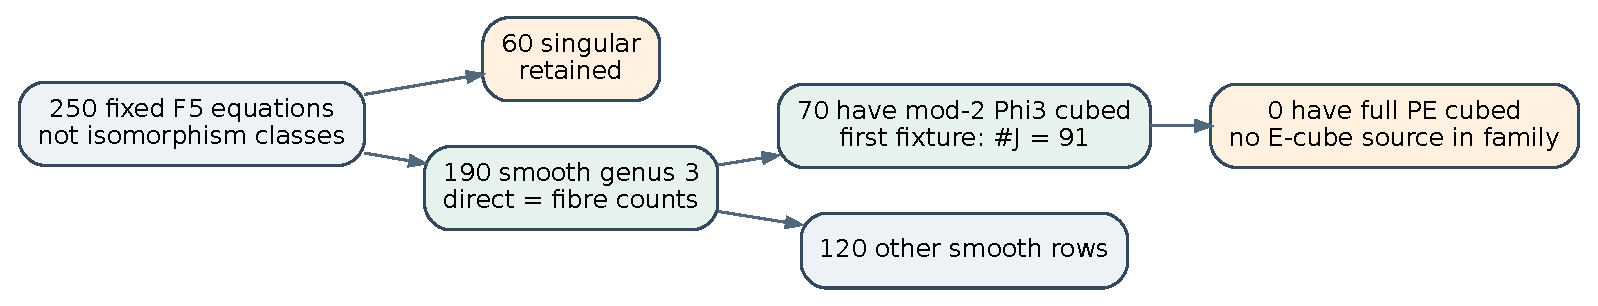
\includegraphics[width=\linewidth,height=58mm,keepaspectratio]{family.pdf}
\end{center}

\textbf{A genuine source, with a different isogeny class.}
The first mod-2 fixture is
\[
 C: Z^4=Y(X^3+2XY^2+Y^3),\qquad (N_1,N_2,N_3)=(5,29,68).
\]
Its Weil polynomial, in ascending coefficient order, is
\[
 [125,-25,10,-21,2,-1,1],\qquad \#J(C)(\mathbf F_5)=91.
\]
It has the original elliptic quotient $v^2=x^3+2x+1$, with factor
$P_E=T^2+T+5$. The complementary factor has ascending coefficients
$[25,-10,-1,-2,1]$. This is not an $E^3$ source.

\textbf{What the mod-2 condition says.}
Every simple Frobenius-module factor has even degree, so every stable
$J[2]$ subspace has even dimension. Multiplication $[2]$ therefore cannot
start with a rational $(2,2,2)$ map on these candidates. This is a written
module argument. It constructs no nontrivial mixed kernel and supplies no
computational advantage or compiled generic Mathlib theorem.

\textbf{Evidence.} Source \texttt{b23c6582}; result \texttt{893f8806};
unsigned claim \texttt{PCC-20261123-d89c72}.
The complete 250 rows, including every singular equation, are retained in
\texttt{first-C-native/quartics.stdout}. [pcc:unverified]
\newpage
{\Large\bfseries Exact gates, failures and remaining bridges}\par

\begin{center}
\begin{tabular}{@{}lr@{}}
\toprule
Fixed equations & 250\\
Smooth / singular & 190 / 60\\
Mod-2 $\Phi_3^3$ / full $P_E^3$ & 70 / 0\\
Strict phases / nonzero exits & 7 / 0\\
Post-call guard failures & 0\\
\bottomrule
\end{tabular}
\end{center}

\textbf{Independent exact controls.}
For all 125 quadratic forms, polynomial gcd and independent Sylvester
matrix rank agree on smoothness. The prescribed $g=0$ positive and
$g=x+1$ actual singular-point negative pass. For every smooth equation,
direct quartic evaluation and elliptic-fibre enumeration agree on all
projective points over $\mathbf F_5,\mathbf F_{25},\mathbf F_{125}$.
All native field pairs and triples, nonzero inverses and Frobenius laws pass.

Newton identities give an integral reciprocal degree-six polynomial.
Every smooth row has exact integer factor $P_E$. Altering $N_3$ by $+3$
rejects that factor, and restoring the original counts restores it. Paired
$\kappa$ counts sum to 14 and 224 in degrees 1 and 3, and agree in degree 2.
No $P_E^3$ row is present; its expected counts would have been $(9,53,84)$.

\textbf{Implementation negatives preserved.}
The first strict format check failed with a complete 5282-byte diagnostic.
The successor copied rustfmt's filename heading into source and failed its
parser with a complete 359-byte diagnostic. Neither reached compilation.
C removes only that prefix from the formatted body. Original sources and
both failures remain immutable. No suppression, population retuning or
resource increase was used.

\textbf{Execution and custody.}
Rust 1.99.1, edition 2021, warnings denied, overflow and debug assertions;
one worker, 2 GiB address space and 120 seconds per phase. All 21 complete
locked inputs were read back before the call. All 38 small original C
records are public, and all 43 result-commit files were read back exactly.
The original 4585568-byte ELF remains in temporary custody pending approved
store or CI retention. This is a development correctness qualification,
not independent replay, a timed comparison or a cryptographic-size solve.

\textbf{Next mathematical gate.}
Ritzenthaler's 2010 primary CM19 example provides a separately motivated
single F7 quartic. Its field, twist, smoothness and point counts require a
separate frozen qualification. It does not replace this F5 negative.
Actual polarized $J[4]$ arithmetic, a nontrivial kernel and quotient map,
target-Jacobian/Serre descent and original elliptic subgroup preservation
remain open. Complete cold costs must include the strongest direct ECDLP
reference and every transfer/setup/solve/replay phase.

\textbf{Sources and standing.}
\href{https://github.com/isogeny-labs/crypto/tree/b23c6582437e3e91d64690aedaf5481ad0ede025/research/chained_genus3_quartic_20261123}{Complete frozen source/protocol}
and
\href{https://github.com/isogeny-labs/crypto/tree/893f88068b6145dec9906a85d6582e5567a3e9b8/research/chained_genus3_quartic_20261123}{full result/raw records}.
Primary review: Ritzenthaler, DOI 10.1112/S1461157009000576, Example 1;
Alekseenko et al., arXiv:0902.1901v2. KB/Conductor unavailable; no novelty
clearance. Existing paid, vault, experiment, formal, CI and merge gates
remain binding. All scientific findings are unsigned. [pcc:unverified]
\end{document}
